\begin{figure*}
\begin{subfigure}{0.34\textwidth}
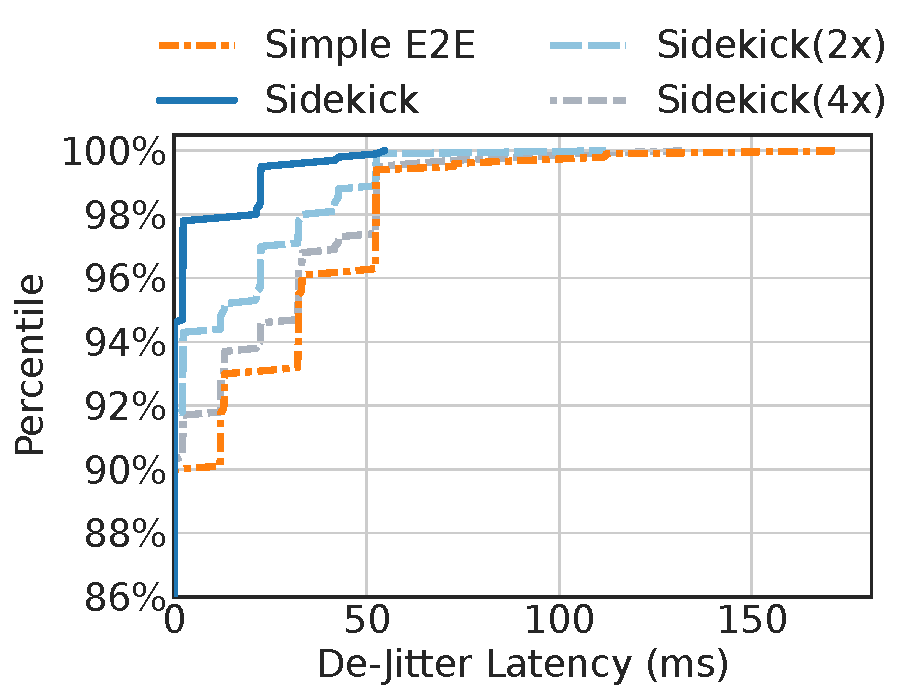
\includegraphics[width=\linewidth]{sidekick/figures/fig4a_low_latency_media_quack.pdf}
\caption{Scenario \#1.}
\label{fig:sidekick:quack-interval:media}
\end{subfigure}
\hfill
\begin{subfigure}{0.31\textwidth}
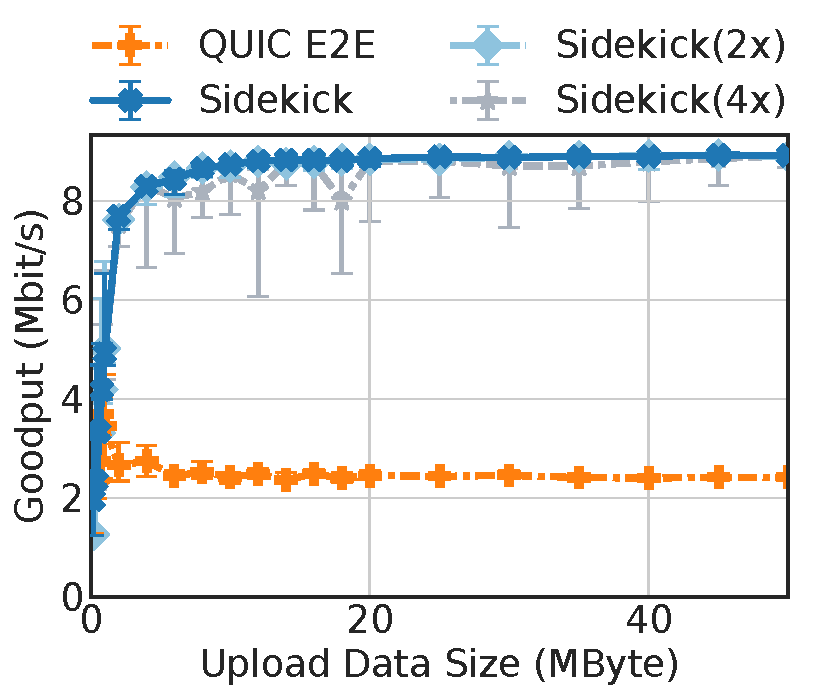
\includegraphics[width=0.97\linewidth]{sidekick/figures/fig4b_pep_emulation_quack.pdf}
\caption{Scenario \#2.
}
\label{fig:sidekick:quack-interval:pep-emulation}
\end{subfigure}
\hfill
\begin{subfigure}{0.32\textwidth}
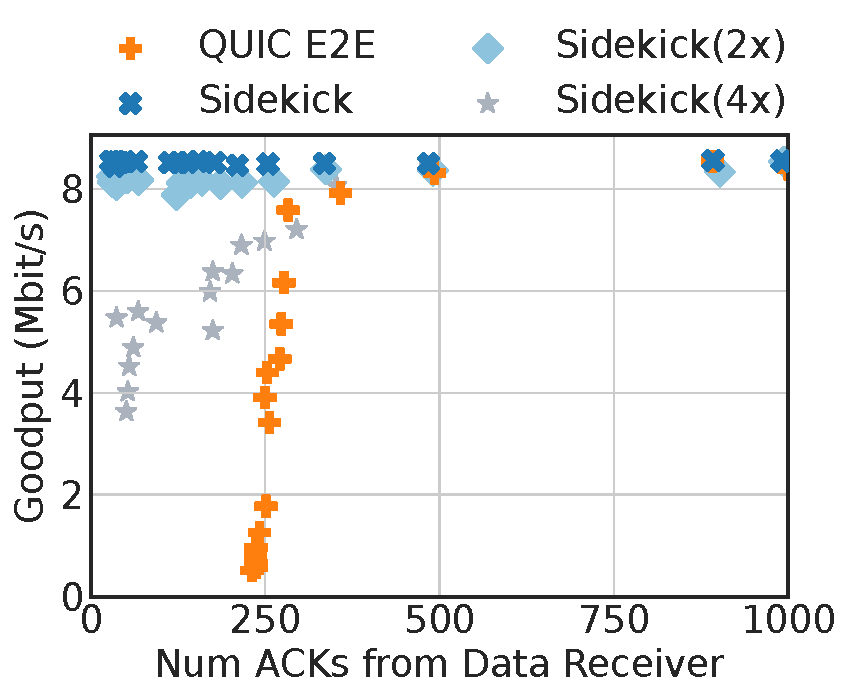
\includegraphics[width=0.99\linewidth]{sidekick/figures/fig4c_ack_reduction_quack.pdf}
\caption{Scenario \#3.}
\label{fig:sidekick:quack-interval:ack-reduction}
\end{subfigure}
\caption{Extending \Cref{fig:sidekick:main-results},
the \textsf{Sidekick($N$x)} data points show
the performance at $N$x the quACK interval (sent less frequently) and
threshold of the default configurations specified in
\Cref{tab:sidekick:experimental-scenarios}.
}
% \dm{Maybe a notation like $x/4$ would be more suggestive than $4x$?}
\label{fig:sidekick:quack-interval}
\end{figure*}
